\section{Overview}

Some fundamental decision had to be made in the early stages of the development of this active object search system. The main questions were what commonsense knowledge can be used to execute the object search intelligently, what information the robot should gather and what sensors are needed for that, how the gathered knowledge about the environment should be represented, and how the search planning, using this knowledge, should be done. 

Indoor environments can be segmented into rooms and room areas, which serve specific purposes, like a kitchen is used for cooking. Therefore the objects located in an area correlate with the type of the area. This connection is used in this work to make the search intelligent and therefore more efficient. Furthermore, knowledge to recognize objects of the searched type and to classify areas into room types is needed. Neural networks, trained on thousands of images, are used, which contain this knowledge in their learned weights.

An RGBD-camera is used to gather the images for the neural networks. The additional depth information is helpful to estimate the positions of the detected objects in space, as this would be difficult otherwise. The depth measurements are also necessary for 3D obstacle detection and mapping. The camera is mounted fixed on the robot to keep the setup simple. Therefore the positioning of the camera is only possible by the two dimensional movement of the robot. As the depth data of the RGBD-camera is not very accurate, a light detection and ranging sensor (LIDAR) is also mounted on the robot. Together with the odometry data from the robot it is used for 2D simultaneous localization and mapping (SLAM). Finally, the robot is equipped with a second RGBD-camera, which is used for the detection of doorways. 

A hybrid map is used to represent the environment. In this hybrid map each room has its own semantic metric map. These room maps consists of multiple maps for the same space, each containing different information. These maps are 
\begin{itemize}
 \item a metric 2D occupancy map for navigation
 \item a 3D occupancy map to avoid obstacles, which are not visible in the LIDAR scans, and for the estimation of likely object locations
 \item a 2D grid map containing the probability distribution over the detectable room types for every grid cell
 \item a 3D grid map for every detectable object type containing the probability that an object of the given type has been seen in a grid cell
\end{itemize}
Furthermore, locations of detected doorways are inserted into the map. The above mentioned maps and the commonsense knowledge are combined to estimate likely object locations. This results in a 3D grid map containing the probabilities of an object of the searched type being in a grid cell. 

On the other hand a topological map is created with a node for every discovered room. These nodes contain references to the corresponding room maps and also additional data. This additional data consists of the estimated time to fully search the room, the probability of an object being in the room and the expected time spent searching in the room for every object type, and estimates for the time needed to leave or traverse a room. If two rooms are connected by a doorway, an edge exists between the corresponding nodes. Figure \ref{fig:topological map} shows an example of such a topological map. 

\begin{figure} 
  \centering
    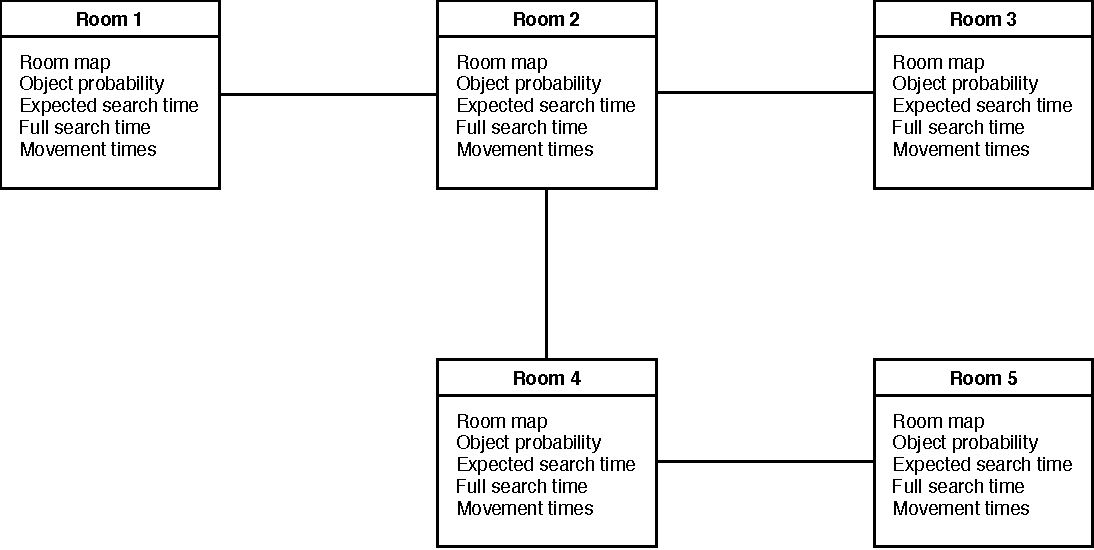
\includegraphics[width=0.8\textwidth]{figures/HybridMap.pdf} 
  \caption[Topological map example]{Example of a topological map with 5 rooms and 4 doorways}
  \label{fig:topological map}
\end{figure}

The goal of the planning is to minimize the expected search time. As the generation of the optimal next search pose given the available information is infeasible, a heuristic is needed. In this work the planning problem is split into two parts. The high-level planner selects the optimal next room to search. It also generates high-level tasks, like move through a doorway, explore room or search room. Based on the pending high-level tasks the low level planner generates the best next goal pose for the robot. Figure \ref{fig:planning} shows a flowchart depicting the general planning procedure. This planner design fits perfectly to the hybrid map as the high-level planner does its planning only on the topological map, while the low-level planner operates only on the room map of the current room. 

\begin{figure}
  \centering
    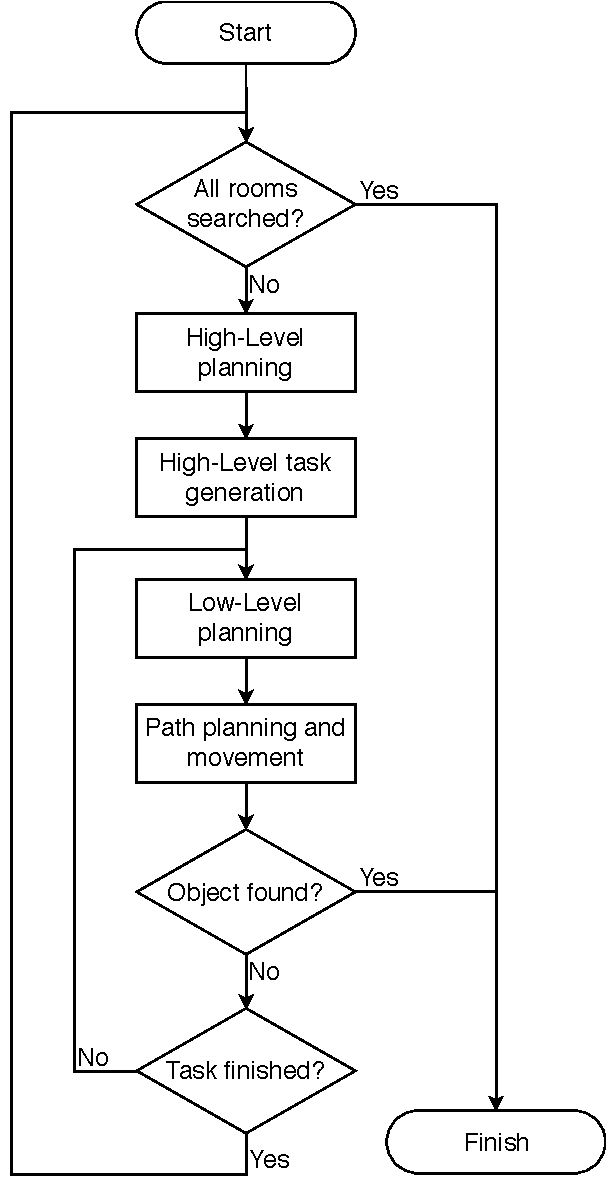
\includegraphics[width=0.4\textwidth]{figures/PlanningFlowChart.pdf} 
  \caption{Flowchart of the planning procedure}
  \label{fig:planning}
\end{figure}

Figure \ref{fig:Overview} gives an overview over the structure of this intelligent active object search system, showing the main components of the system and also the most important data exchanged by these components.

\begin{figure}
  \centering
    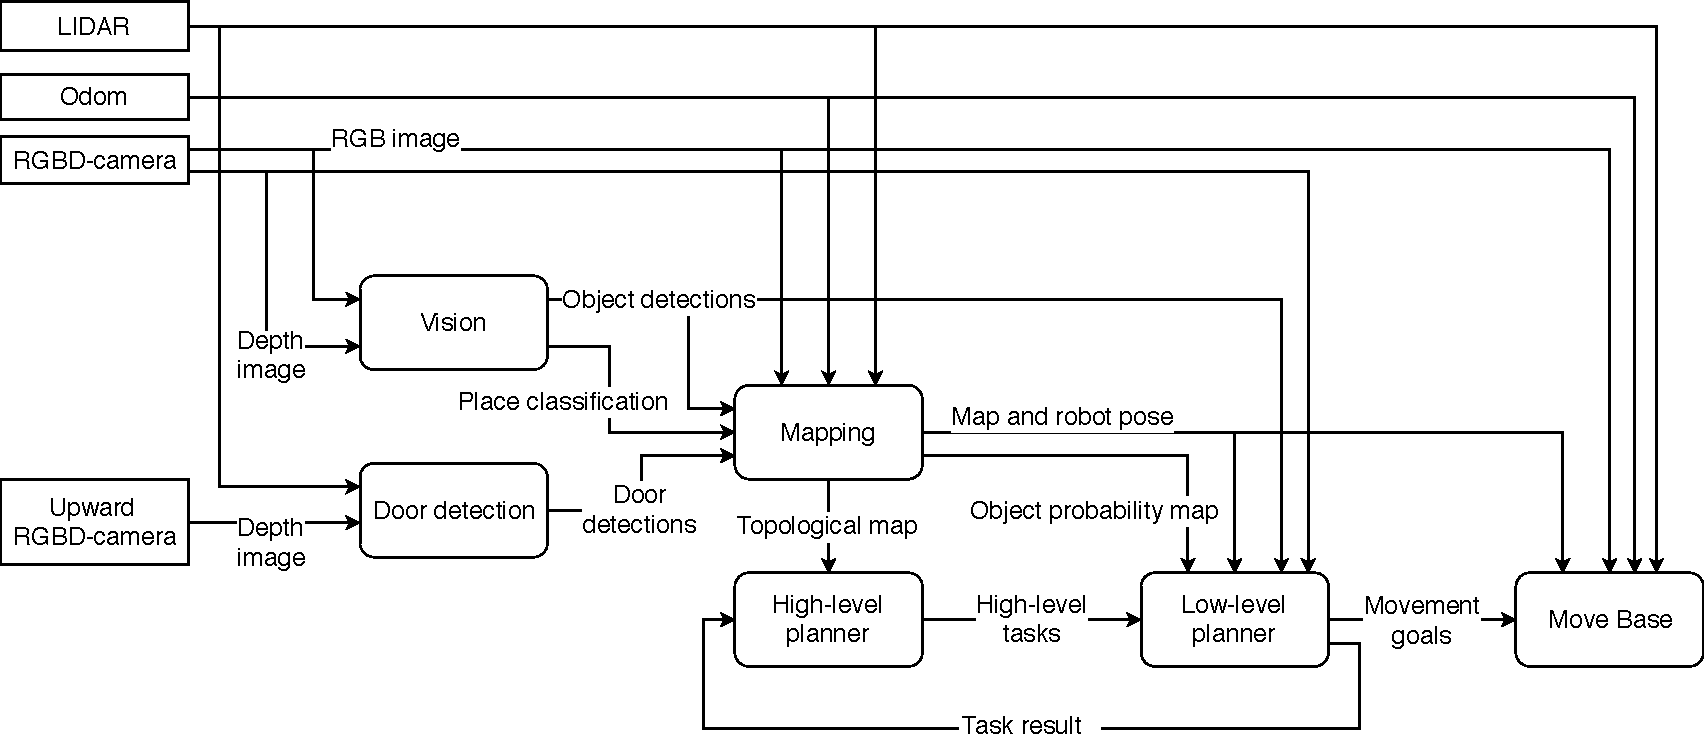
\includegraphics[width=1.0\textwidth]{figures/Overview.pdf} 
  \caption{Overview over the full system structure}
  \label{fig:Overview}
\end{figure}
